\documentclass[aspectratio=169]{beamer}
\usetheme{Madrid}
\usecolortheme{default}

% Modern color scheme
\definecolor{primaryblue}{RGB}{41, 128, 185}
\definecolor{darkblue}{RGB}{52, 73, 94}
\definecolor{lightgray}{RGB}{236, 240, 241}
\definecolor{darkgray}{RGB}{52, 73, 94}
\definecolor{accent}{RGB}{231, 76, 60}
\definecolor{success}{RGB}{46, 204, 113}
\definecolor{warning}{RGB}{241, 196, 15}

% Set theme colors
\setbeamercolor{structure}{fg=primaryblue}
\setbeamercolor{palette primary}{bg=primaryblue,fg=white}
\setbeamercolor{palette secondary}{bg=darkblue,fg=white}
\setbeamercolor{palette tertiary}{bg=lightgray,fg=darkgray}
\setbeamercolor{palette quaternary}{bg=darkgray,fg=white}
\setbeamercolor{frametitle}{bg=primaryblue,fg=white}
\setbeamercolor{title}{fg=darkblue}
\setbeamercolor{block title}{bg=primaryblue,fg=white}
\setbeamercolor{block body}{bg=lightgray,fg=darkgray}
\setbeamercolor{block title alerted}{bg=accent,fg=white}
\setbeamercolor{block body alerted}{bg=accent!10,fg=darkgray}

% Remove navigation symbols
\setbeamertemplate{navigation symbols}{}

% Modern frame title
\setbeamertemplate{frametitle}{
    \begin{beamercolorbox}[wd=\paperwidth,ht=2.5ex,dp=1ex,leftskip=1em,rightskip=1em]{frametitle}
        \usebeamerfont{frametitle}\insertframetitle
    \end{beamercolorbox}
}

% Modern itemize
\setbeamertemplate{itemize items}[circle]
\setbeamercolor{itemize item}{fg=primaryblue}
\setbeamercolor{itemize subitem}{fg=darkblue}
\setbeamercolor{enumerate item}{fg=primaryblue}

\usepackage{listings}
\usepackage{graphicx}
\usepackage{tikz}
\usepackage{amsmath}
\usepackage{amssymb}
\usepackage[ruled,vlined]{algorithm2e}
\usepackage{xcolor}

\usetikzlibrary{shapes,arrows,positioning,calc}

\lstset{
  language=SQL,
  basicstyle=\ttfamily\footnotesize,
  keywordstyle=\color{primaryblue}\bfseries,
  commentstyle=\color{success}\itshape,
  stringstyle=\color{accent},
  showstringspaces=false,
  frame=single,
  frameround=tttt,
  rulecolor=\color{lightgray},
  backgroundcolor=\color{lightgray},
  breaklines=true,
  numbers=left,
  numberstyle=\tiny\color{darkgray},
  stepnumber=1,
  numbersep=8pt,
  tabsize=2,
  columns=flexible,
  keepspaces=true,
}

\title{\textbf{pyHMSSQL}}
\subtitle{Teljes Adatbázis-kezelő Rendszer\\Architektúra, Elmélet és Végrehajtási Pipeline}
\author{\textbf{Adatbázis Rendszerek Analízis}}
\institute{Haladó Adatbázis Rendszerek}
\date{\today}

% Modern title page
\setbeamertemplate{title page}{
    \begin{center}
        \vspace{1cm}
        {\usebeamerfont{title}\usebeamercolor[fg]{title}\inserttitle\par}
        \vspace{0.5cm}
        {\usebeamerfont{subtitle}\usebeamercolor[fg]{subtitle}\insertsubtitle\par}
        \vspace{1cm}
        {\usebeamerfont{author}\insertauthor\par}
        \vspace{0.3cm}
        {\usebeamerfont{institute}\insertinstitute\par}
        \vspace{0.5cm}
        {\usebeamerfont{date}\insertdate\par}
    \end{center}
}

\begin{document}

\frame{\titlepage}

\begin{frame}{Tartalom}
\tableofcontents[hideallsubsections]
\end{frame}

\section{Bevezetés és Rendszer Áttekintés}

\begin{frame}{Mi a pyHMSSQL?}
\begin{columns}
\begin{column}{0.6\textwidth}
\begin{itemize}
    \item \textbf{Teljes DBMS Implementáció} Python nyelven
    \item \textbf{Kliens-Szerver Architektúra} socket-alapú kommunikációval
    \item \textbf{Egyedi B+ Fa Indexelés} hatékony adatlekérdezéshez
    \item \textbf{Teljes SQL Támogatás} beleértve összetett lekérdezések, összekapcsolások, tranzakciók
    \item \textbf{Haladó Funkciók}: Nézetek, tárolt eljárások, triggerek, replikáció
    \item \textbf{Többféle Felület}: CLI, GUI (JavaFX), REST API
\end{itemize}
\end{column}
\begin{column}{0.35\textwidth}
\begin{alertblock}{Fő Innováció}
A legtöbb akadémiai DBMS projekttel ellentétben, a pyHMSSQL \textbf{gyártásra kész funkciókat} implementál, beleértve ACID tranzakciókat, idegen kulcs megszorításokat, lekérdezés optimalizálást és elosztott replikációt.
\end{alertblock}
\end{column}
\end{columns}
\end{frame}

\begin{frame}{Rendszer Architektúra Áttekintés}
\begin{center}
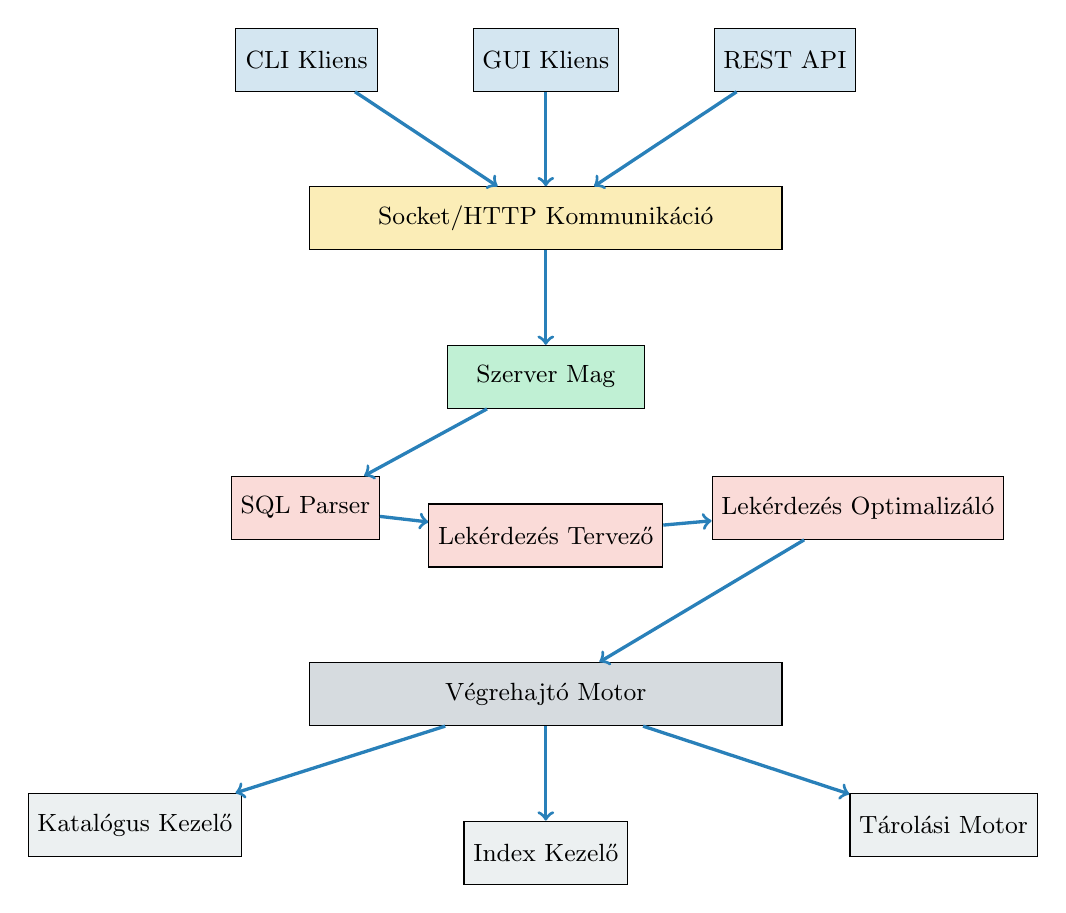
\begin{tikzpicture}[node distance=1.2cm, every node/.style={font=\small}]
    % Client Layer
    \node[rectangle, draw, fill=primaryblue!20, minimum width=1.8cm, minimum height=0.8cm] (cli) {CLI Kliens};
    \node[rectangle, draw, fill=primaryblue!20, minimum width=1.8cm, minimum height=0.8cm, right=of cli] (gui) {GUI Kliens};
    \node[rectangle, draw, fill=primaryblue!20, minimum width=1.8cm, minimum height=0.8cm, right=of gui] (rest) {REST API};
    
    % Communication Layer
    \node[rectangle, draw, fill=warning!30, minimum width=6cm, minimum height=0.8cm, below=of gui] (comm) {Socket/HTTP Kommunikáció};
    
    % Server Core
    \node[rectangle, draw, fill=success!30, minimum width=2.5cm, minimum height=0.8cm, below=of comm] (server) {Szerver Mag};
    
    % Processing Pipeline
    \node[rectangle, draw, fill=accent!20, minimum width=1.6cm, minimum height=0.8cm, below left=of server] (parser) {SQL Parser};
    \node[rectangle, draw, fill=accent!20, minimum width=1.6cm, minimum height=0.8cm, below=of server] (planner) {Lekérdezés Tervező};
    \node[rectangle, draw, fill=accent!20, minimum width=1.6cm, minimum height=0.8cm, below right=of server] (optimizer) {Lekérdezés Optimalizáló};
    
    % Execution Engine
    \node[rectangle, draw, fill=darkblue!20, minimum width=6cm, minimum height=0.8cm, below=of planner] (engine) {Végrehajtó Motor};
    
    % Storage Layer
    \node[rectangle, draw, fill=lightgray, minimum width=1.6cm, minimum height=0.8cm, below left=of engine] (catalog) {Katalógus Kezelő};
    \node[rectangle, draw, fill=lightgray, minimum width=1.6cm, minimum height=0.8cm, below=of engine] (index) {Index Kezelő};
    \node[rectangle, draw, fill=lightgray, minimum width=1.6cm, minimum height=0.8cm, below right=of engine] (storage) {Tárolási Motor};
    
    % Modern arrows
    \draw[->, line width=1.2pt, color=primaryblue] (cli) -- (comm);
    \draw[->, line width=1.2pt, color=primaryblue] (gui) -- (comm);
    \draw[->, line width=1.2pt, color=primaryblue] (rest) -- (comm);
    \draw[->, line width=1.2pt, color=primaryblue] (comm) -- (server);
    \draw[->, line width=1.2pt, color=primaryblue] (server) -- (parser);
    \draw[->, line width=1.2pt, color=primaryblue] (parser) -- (planner);
    \draw[->, line width=1.2pt, color=primaryblue] (planner) -- (optimizer);
    \draw[->, line width=1.2pt, color=primaryblue] (optimizer) -- (engine);
    \draw[->, line width=1.2pt, color=primaryblue] (engine) -- (catalog);
    \draw[->, line width=1.2pt, color=primaryblue] (engine) -- (index);
    \draw[->, line width=1.2pt, color=primaryblue] (engine) -- (storage);
\end{tikzpicture}
\end{center}
\end{frame}

\section{Lekérdezés Feldolgozási Pipeline}

\begin{frame}{Lekérdezés Feldolgozási Pipeline Áttekintés}
\begin{center}
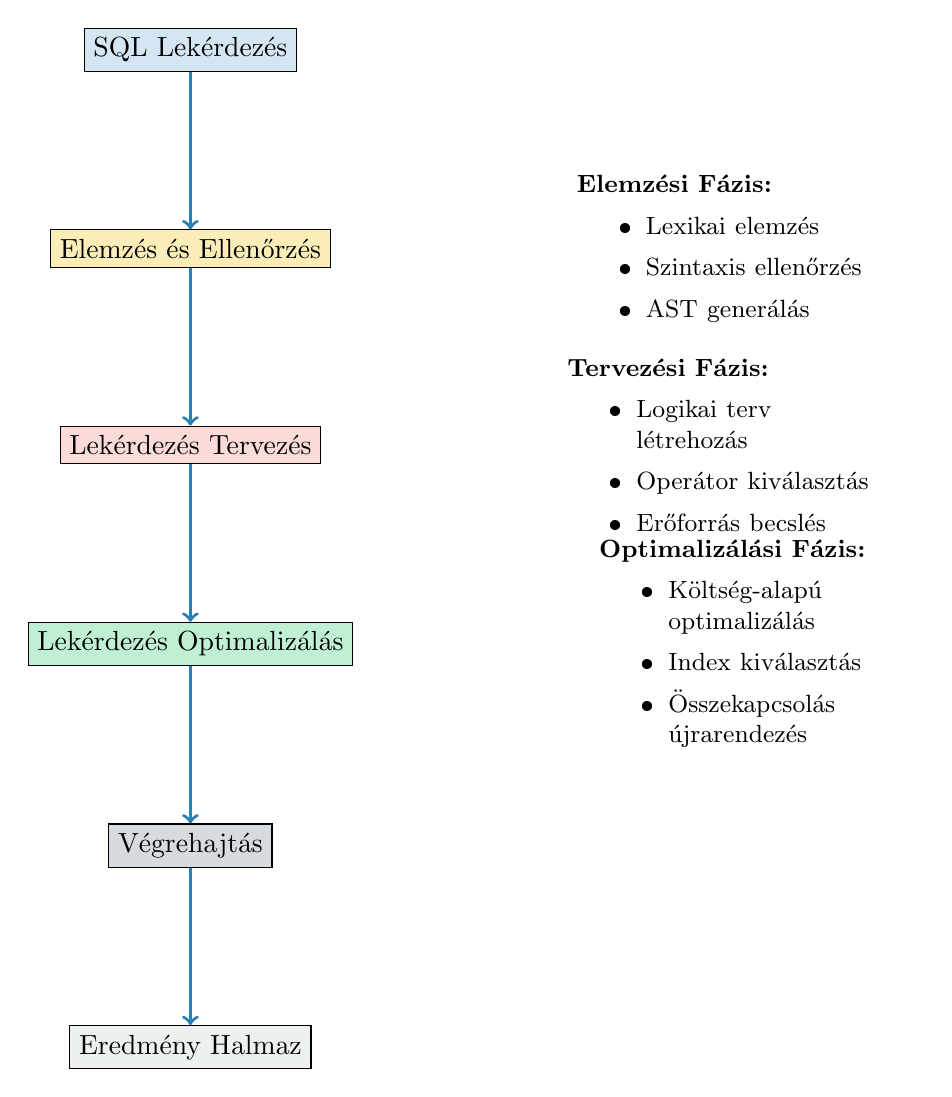
\begin{tikzpicture}[node distance=2cm, auto]
    \node[rectangle, draw, fill=primaryblue!20] (input) {SQL Lekérdezés};
    \node[rectangle, draw, fill=warning!30, below=of input] (parse) {Elemzés és Ellenőrzés};
    \node[rectangle, draw, fill=accent!20, below=of parse] (plan) {Lekérdezés Tervezés};
    \node[rectangle, draw, fill=success!30, below=of plan] (optimize) {Lekérdezés Optimalizálás};
    \node[rectangle, draw, fill=darkblue!20, below=of optimize] (execute) {Végrehajtás};
    \node[rectangle, draw, fill=lightgray, below=of execute] (result) {Eredmény Halmaz};
    
    % Side annotations
    \node[right=3cm of parse, text width=4cm] {
        \small
        \textbf{Elemzési Fázis:}
        \begin{itemize}
            \item Lexikai elemzés
            \item Szintaxis ellenőrzés
            \item AST generálás
        \end{itemize}
    };
    
    \node[right=3cm of plan, text width=4cm] {
        \small
        \textbf{Tervezési Fázis:}
        \begin{itemize}
            \item Logikai terv létrehozás
            \item Operátor kiválasztás
            \item Erőforrás becslés
        \end{itemize}
    };
    
    \node[right=3cm of optimize, text width=4cm] {
        \small
        \textbf{Optimalizálási Fázis:}
        \begin{itemize}
            \item Költség-alapú optimalizálás
            \item Index kiválasztás
            \item Összekapcsolás újrarendezés
        \end{itemize}
    };
    
    \draw[->, line width=1.2pt, color=primaryblue] (input) -- (parse);
    \draw[->, line width=1.2pt, color=primaryblue] (parse) -- (plan);
    \draw[->, line width=1.2pt, color=primaryblue] (plan) -- (optimize);
    \draw[->, line width=1.2pt, color=primaryblue] (optimize) -- (execute);
    \draw[->, line width=1.2pt, color=primaryblue] (execute) -- (result);
\end{tikzpicture}
\end{center}
\end{frame}

\begin{frame}[fragile]{SQL Elemzés és AST Generálás}
\begin{block}{Elemzési Bemenet}
Az elemző az SQL karakterláncokat strukturált lekérdezési tervekké alakítja:
\end{block}

\begin{lstlisting}[language=SQL]
SELECT dept_id, AVG(salary) as avg_salary, COUNT(*) as emp_count 
FROM employees 
GROUP BY dept_id
\end{lstlisting}

\begin{block}{Elemzett Kimenet Struktúra}
\begin{lstlisting}[language=Python]
{
    "type": "AGGREGATE_GROUP",
    "table": "employees",
    "columns": ["dept_id", "AVG(salary)", "COUNT(*)"],
    "group_by": ["dept_id"],
    "aliases": {"AVG(salary)": "avg_salary", "COUNT(*)": "emp_count"},
    "functions": {
        "AVG(salary)": {"function": "AVG", "column": "salary"},
        "COUNT(*)": {"function": "COUNT", "column": "*"}
    }
}
\end{lstlisting}
\end{block}
\end{frame}

\section{Lekérdezés Tervezés és Optimalizálás}

\begin{frame}{Lekérdezés Tervezés Elmélet}
\begin{block}{Logikai vs Fizikai Tervek}
\begin{itemize}
    \item \textbf{Logikai Terv}: Magas szintű műveletek leírása
    \item \textbf{Fizikai Terv}: Konkrét algoritmusok és hozzáférési módszerek
\end{itemize}
\end{block}

\begin{block}{Tervezési Folyamat a pyHMSSQL-ben}
\begin{enumerate}
    \item \textbf{Tábla Ellenőrzés}: Táblák létezésének ellenőrzése kis- és nagybetű különbségtétel nélkül
    \item \textbf{Oszlop Feloldás}: Oszlopok hozzárendelése a valós tábla sémához
    \item \textbf{Operátor Kiválasztás}: Megfelelő végrehajtási operátorok kiválasztása
    \item \textbf{Megszorítás Integráció}: Idegen kulcs és ellenőrzési megszorítások alkalmazása
    \item \textbf{Index Megfontolás}: Elérhető indexek azonosítása optimalizáláshoz
\end{enumerate}
\end{block}

\begin{alertblock}{Haladó Funkció}
A pyHMSSQL támogatja az \textbf{összetett elsődleges kulcsokat} és \textbf{összetett indexeket}, lehetővé téve összetett relációs terveket.
\end{alertblock}
\end{frame}

\begin{frame}{Költség-alapú Lekérdezés Optimalizálás}
\begin{block}{Implementált Optimalizálási Stratégiák}
\begin{enumerate}
    \item \textbf{Index-alapú Hozzáférési Útvonal Kiválasztás}
    \item \textbf{Összekapcsolási Algoritmus Kiválasztás} (Hash, Sort-Merge, Nested Loop, Index)
    \item \textbf{Összekapcsolás Újrarendezés} heurisztikák és költségbecslés alapján
    \item \textbf{Predikátum Lenyomás} köztes eredményméretek csökkentésére
    \item \textbf{Kifejezés Újraírás} és egyszerűsítés
    \item \textbf{Rendezés-Limit Optimalizálás} (Top-N konverzió)
\end{enumerate}
\end{block}

\begin{block}{Költség Modell}
\begin{align}
\text{Költség}_{összes} &= \text{Költség}_{CPU} + \text{Költség}_{I/O} \\
\text{Költség}_{I/O} &= \text{Oldalak}_{olvasott} \times \text{Költség}_{oldal} \\
\text{Költség}_{CPU} &= \text{Rekordok}_{feldolgozott} \times \text{Költség}_{rekord}
\end{align}
\end{block}
\end{frame}

\begin{frame}[fragile]{Index Kiválasztás és Optimalizálás}
\begin{block}{Támogatott Index Típusok}
\begin{itemize}
    \item \textbf{B+ Fa Indexek}: Elsődleges hozzáférési módszer
    \item \textbf{Egyedi Indexek}: Megszorítás kikényszerítés
    \item \textbf{Összetett Indexek}: Többoszlopos indexelés
\end{itemize}
\end{block}

\begin{lstlisting}[language=Python]
# Index létrehozás összetett oszlopokkal
def execute_create_index(self, plan):
    columns = plan.get("columns", [])
    if len(columns) > 1:
        column_key = "_".join(columns)  # Összetett kulcs
        index_display = f"({', '.join(columns)})"
    else:
        column_key = columns[0]
        index_display = columns[0]
        
    # B+ Fa létrehozás összetett kulcs támogatással
    result = self.catalog_manager.create_index(
        table_name=table_name,
        column_name=column_key,
        index_name=index_name,
        is_unique=is_unique,
        columns=columns
    )
\end{lstlisting}
\end{frame}

\section{B+ Fa Implementáció}

\begin{frame}{B+ Fa Elmélet és Implementáció}
\begin{block}{Miért B+ Fák az Adatbázisokhoz?}
\begin{itemize}
    \item \textbf{Kiegyensúlyozott Hozzáférés}: $O(\log n)$ keresés, beszúrás, törlés
    \item \textbf{Tartomány Lekérdezések}: Hatékony szekvenciális hozzáférés levelek összekapcsolásával
    \item \textbf{Magas Elágazási Tényező}: Minimalizálja a fa magasságot, csökkenti I/O-t
    \item \textbf{Perzisztencia}: Optimalizált lemez-alapú tároláshoz
\end{itemize}
\end{block}

\begin{block}{B+ Fa Tulajdonságok}
\begin{itemize}
    \item Minden adat levél csomópontokban tárolva
    \item Belső csomópontok csak navigációs kulcsokat tárolnak
    \item Levél csomópontok összekapcsolva szekvenciális hozzáféréshez
    \item Kiegyensúlyozottság fenntartása csomópont hasítás/összeolvasztás révén
\end{itemize}
\end{block}

\begin{alertblock}{Implementációs Részlet}
A pyHMSSQL B+ Fája támogatja a \textbf{szerializációt} perzisztenciához és \textbf{összetett kulcsokat} többoszlopos indexekhez.
\end{alertblock}
\end{frame}

\begin{frame}{B+ Fa Műveletek}
\begin{center}
\begin{tikzpicture}[level distance=1.5cm, sibling distance=3cm]
    \node[rectangle, draw] {50}
        child {
            node[rectangle, draw] {25}
            child {node[rectangle, draw] {10, 20}}
            child {node[rectangle, draw] {30, 40}}
        }
        child {
            node[rectangle, draw] {75}
            child {node[rectangle, draw] {60, 70}}
            child {node[rectangle, draw] {80, 90}}
        };
    
    % Leaf links
    \draw[->] (3.5,-2.7) -- (6.5,-2.7);
    \draw[->] (6.5,-2.7) -- (9.5,-2.7);
    \draw[->] (9.5,-2.7) -- (12.5,-2.7);
\end{tikzpicture}
\end{center}

\begin{block}{Keresési Algoritmus Komplexitás}
\begin{align}
\text{Magasság} &= \lceil \log_{\text{elágazási tényező}} n \rceil \\
\text{Keresési Költség} &= \text{Magasság} \times \text{Költség}_{oldal\_olvasás} \\
\text{Tartomány Költség} &= \text{Keresési Költség} + k \times \text{Költség}_{szekvenciális}
\end{align}
ahol $k$ a kvalifikáló rekordok száma.
\end{block}
\end{frame}

\section{Végrehajtó Motor Architektúra}

\begin{frame}{Végrehajtó Motor Komponensei}
\begin{center}
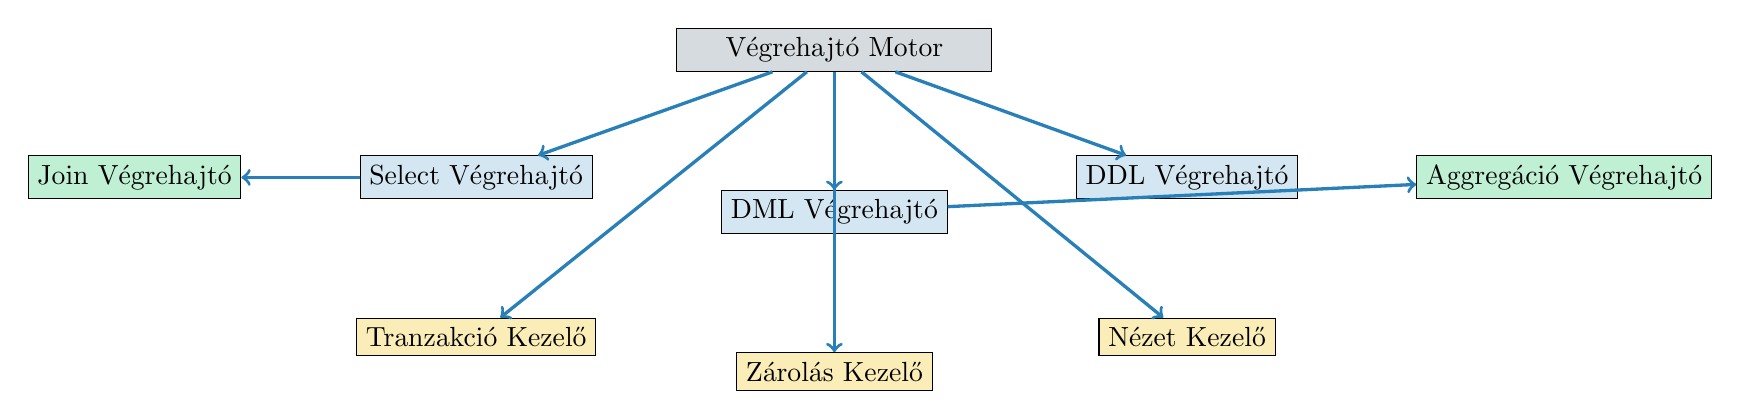
\begin{tikzpicture}[node distance=1.5cm]
    % Main Engine
    \node[rectangle, draw, fill=darkblue!20, minimum width=4cm] (engine) {Végrehajtó Motor};
    
    % Sub-executors
    \node[rectangle, draw, fill=primaryblue!20, below left=of engine] (select) {Select Végrehajtó};
    \node[rectangle, draw, fill=primaryblue!20, below=of engine] (dml) {DML Végrehajtó};
    \node[rectangle, draw, fill=primaryblue!20, below right=of engine] (ddl) {DDL Végrehajtó};
    
    % Specialized components
    \node[rectangle, draw, fill=success!30, left=of select] (join) {Join Végrehajtó};
    \node[rectangle, draw, fill=success!30, right=of ddl] (agg) {Aggregáció Végrehajtó};
    
    % Support systems
    \node[rectangle, draw, fill=warning!30, below=of select] (trans) {Tranzakció Kezelő};
    \node[rectangle, draw, fill=warning!30, below=of dml] (lock) {Zárolás Kezelő};
    \node[rectangle, draw, fill=warning!30, below=of ddl] (view) {Nézet Kezelő};
    
    % Arrows
    \draw[->, line width=1.2pt, color=primaryblue] (engine) -- (select);
    \draw[->, line width=1.2pt, color=primaryblue] (engine) -- (dml);
    \draw[->, line width=1.2pt, color=primaryblue] (engine) -- (ddl);
    \draw[->, line width=1.2pt, color=primaryblue] (select) -- (join);
    \draw[->, line width=1.2pt, color=primaryblue] (dml) -- (agg);
    \draw[->, line width=1.2pt, color=primaryblue] (engine) -- (trans);
    \draw[->, line width=1.2pt, color=primaryblue] (engine) -- (lock);
    \draw[->, line width=1.2pt, color=primaryblue] (engine) -- (view);
\end{tikzpicture}
\end{center}
\end{frame}

\begin{frame}[fragile]{Végrehajtó Motor Küldési Logika}
\begin{lstlisting}[language=Python]
def execute(self, plan):
    """Fő végrehajtási küldő"""
    plan_type = plan.get("type", "UNKNOWN")
    
    if plan_type == "SELECT":
        return self.select_executor.execute_select(plan)
    elif plan_type == "INSERT":
        return self.dml_executor.execute_insert(plan)
    elif plan_type == "UPDATE":
        return self.dml_executor.execute_update(plan)
    elif plan_type == "DELETE":
        return self.dml_executor.execute_delete(plan)
    elif plan_type == "JOIN":
        return self.join_executor.execute_join(plan)
    elif plan_type == "AGGREGATE":
        return self.aggregate_executor.execute_aggregate(plan)
    elif plan_type == "AGGREGATE_GROUP":
        return self.execute_aggregate_with_groupby(plan)
    elif plan_type in ["UNION", "INTERSECT", "EXCEPT"]:
        return self.execute_set_operation(plan)
    elif plan_type == "BATCH_INSERT":
        return self.execute_batch_insert(plan)
    # ... további operátorok
\end{lstlisting}
\end{frame}

\section{Adatmanipulációs Nyelv (DML)}

\begin{frame}{DML Műveletek Elmélete}
\begin{block}{ACID Tulajdonságok Implementációja}
\begin{itemize}
    \item \textbf{Atomicitás}: Tranzakció-alapú műveletek visszavonási képességgel
    \item \textbf{Konzisztencia}: Idegen kulcs megszorítás kikényszerítés
    \item \textbf{Izolációs szint}: Zárolás-alapú egyidejűség-vezérlés
    \item \textbf{Tartósság}: Perzisztens tárolás előre írt naplózással
\end{itemize}
\end{block}

\begin{block}{Megszorítás Kikényszerítés}
\begin{itemize}
    \item \textbf{Elsődleges Kulcs}: Egyediség és nem-null ellenőrzés
    \item \textbf{Idegen Kulcs}: Referenciális integritás ellenőrzés
    \item \textbf{Ellenőrzési Megszorítások}: Tartomány validáció
    \item \textbf{Egyediségi Megszorítások}: Duplikátum megelőzés
\end{itemize}
\end{block}
\end{frame}

\begin{frame}[fragile]{Idegen Kulcs Megszorítás Kikényszerítés}
\begin{lstlisting}[language=Python]
def _check_fk_constraints_for_delete(self, db_name, table_name, records_to_delete):
    """Ellenőrzi, hogy a törlés sérti-e a referenciális integritást"""
    
    # Minden tábla megkeresése, amely hivatkozhat erre a táblára
    tables = self.catalog_manager.list_tables(db_name)
    
    for other_table in tables:
        if other_table == table_name:
            continue
            
        # Idegen kulcs kapcsolatok kibontása a sémából
        schema = self.catalog_manager.get_table_schema(other_table)
        fk_relationships = self._extract_foreign_keys(schema)
        
        for relationship in fk_relationships:
            if relationship['referenced_table'] == table_name:
                # Ellenőrzi, hogy léteznek-e hivatkozó rekordok
                for record in records_to_delete:
                    ref_value = record[relationship['referenced_column']]
                    
                    referencing_records = self.catalog_manager.query_with_condition(
                        other_table, 
                        [{"column": relationship['foreign_key_column'], 
                          "operator": "=", 
                          "value": ref_value}], 
                        ["*"]
                    )
                    
                    if referencing_records:
                        return f"FK megszorítás sértés: {other_table} hivatkozik {table_name}-ra"
    
    return None  # Nincs sértés
\end{lstlisting}
\end{frame}

\begin{frame}{Kötegelt Műveletek és Teljesítmény}
\begin{block}{Kötegelt Beszúrás Optimalizálás}
\begin{itemize}
    \item \textbf{Köteg Méret Hangolás}: Alapértelmezett 5000 rekord kötegenként
    \item \textbf{Index Karbantartás}: Halasztva a köteg befejezéséig
    \item \textbf{Memória Kezelés}: Folyamatos feldolgozás nagy adathalmazokhoz
    \item \textbf{Hibakezelés}: Részleges sikeresség jelentés
\end{itemize}
\end{block}

\begin{block}{Teljesítmény Metrikák}
\begin{align}
\text{Áteresztőképesség} &= \frac{\text{Beszúrt Rekordok}}{\text{Összes Idő}} \\
\text{Köteg Hatékonyság} &= \frac{\text{Kötegelt Beszúrás Idő}}{\text{Egyedi Beszúrás Idő} \times \text{Köteg Méret}}
\end{align}
\end{block}

\begin{alertblock}{Valós Teljesítmény}
A kötegelt beszúrások \textbf{10-100x} teljesítményjavulást érnek el az egyedi beszúrásokhoz képest a csökkentett költségek és optimalizált index frissítések miatt.
\end{alertblock}
\end{frame}

\section{Összekapcsolási Algoritmusok}

\begin{frame}{Összekapcsolási Algoritmus Kiválasztás}
\begin{block}{Elérhető Összekapcsolási Algoritmusok}
\begin{enumerate}
    \item \textbf{Hash Join}: Alapértelmezett egyenlőségi összekapcsolásokhoz
    \item \textbf{Sort-Merge Join}: Rendezett bemenetekhez
    \item \textbf{Nested Loop Join}: Tartalék algoritmus
    \item \textbf{Index Join}: Amikor indexek elérhetők
\end{enumerate}
\end{block}

\begin{block}{Algoritmus Kiválasztási Kritériumok}
\begin{itemize}
    \item \textbf{Tábla Méret}: Hash join nagy táblákhoz
    \item \textbf{Index Elérhetőség}: Index join amikor megfelelő indexek léteznek
    \item \textbf{Join Szelektivitás}: Nested loop nagyon szelektív összekapcsolásokhoz
    \item \textbf{Memória Megszorítások}: Sort-merge memória-korlátozott környezetekhez
\end{itemize}
\end{block}
\end{frame}

\begin{frame}{Hash Join Implementáció}
\begin{center}
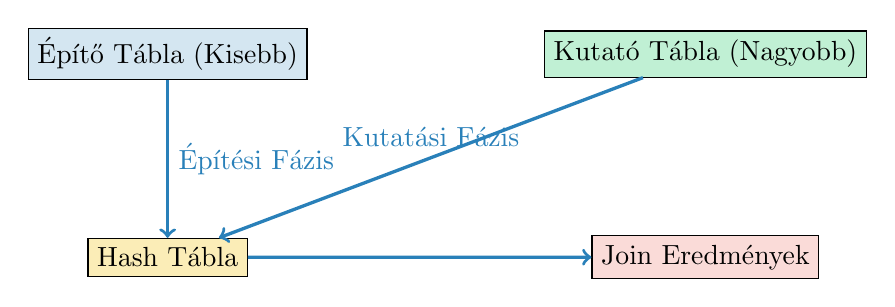
\begin{tikzpicture}[node distance=2cm]
    % Build Phase
    \node[rectangle, draw, fill=primaryblue!20] (build_table) {Építő Tábla (Kisebb)};
    \node[rectangle, draw, fill=warning!30, below=of build_table] (hash_table) {Hash Tábla};
    
    % Probe Phase
    \node[rectangle, draw, fill=success!30, right=3cm of build_table] (probe_table) {Kutató Tábla (Nagyobb)};
    \node[rectangle, draw, fill=accent!20, below=of probe_table] (join_result) {Join Eredmények};
    
    % Process
    \draw[->, line width=1.2pt, color=primaryblue] (build_table) -- (hash_table) node[midway, right] {Építési Fázis};
    \draw[->, line width=1.2pt, color=primaryblue] (probe_table) -- (hash_table) node[midway, above] {Kutatási Fázis};
    \draw[->, line width=1.2pt, color=primaryblue] (hash_table) -- (join_result);
\end{tikzpicture}
\end{center}

\begin{block}{Hash Join Komplexitás}
\begin{align}
\text{Építési Költség} &= |R| \times \text{Költség}_{hash} \\
\text{Kutatási Költség} &= |S| \times \text{Költség}_{keresés} \\
\text{Összes Költség} &= |R| + |S| + \text{Kimenet Méret}
\end{align}
ahol $|R|$ az építő reláció mérete és $|S|$ a kutató reláció mérete.
\end{block}
\end{frame}

\begin{frame}[fragile]{Join Végrehajtás Tippekkel}
\begin{lstlisting}[language=Python]
def execute_join(self, plan):
    """Join végrehajtás algoritmus kiválasztással"""
    
    # Join tipp kibontása a tervből
    join_hint = plan.get("hint", {}).get("JOIN_TYPE", "HASH")
    left_table = plan.get("left_table")
    right_table = plan.get("right_table")
    join_condition = plan.get("condition")
    
    # Join algoritmus kiválasztás tipp és statisztikák alapján
    if join_hint == "HASH" or self._should_use_hash_join(left_table, right_table):
        return self._execute_hash_join(plan)
    elif join_hint == "MERGE" or self._should_use_sort_merge(left_table, right_table):
        return self._execute_sort_merge_join(plan)
    elif join_hint == "INDEX" and self._has_suitable_index(join_condition):
        return self._execute_index_join(plan)
    else:
        return self._execute_nested_loop_join(plan)

def _should_use_hash_join(self, left_table, right_table):
    """Költség-alapú döntés hash join-hoz"""
    left_size = self.catalog_manager.get_table_size(left_table)
    right_size = self.catalog_manager.get_table_size(right_table)
    
    # Hash join használata ha az egyik tábla jelentősen kisebb
    return min(left_size, right_size) * 10 < max(left_size, right_size)
\end{lstlisting}
\end{frame}

\section{Aggregáció és Csoportosítás}

\begin{frame}{Aggregáció Elmélet}
\begin{block}{Implementált Aggregációs Függvények}
\begin{itemize}
    \item \textbf{Standard Függvények}: COUNT, SUM, AVG, MIN, MAX
    \item \textbf{Matematikai Függvények}: GCD (Legnagyobb Közös Osztó)
    \item \textbf{Mintavételezési Függvények}: RAND paraméteres mintavételezéssel
\end{itemize}
\end{block}

\begin{block}{Csoportosítás Implementációs Stratégia}
\begin{enumerate}
    \item \textbf{Csoportosítási Fázis}: Hash-alapú particionálás csoport kulcs szerint
    \item \textbf{Aggregációs Fázis}: Aggregáció függvények alkalmazása csoportonként
    \item \textbf{Eredmény Összeállítás}: Csoport kulcsok kombinálása aggregált értékekkel
\end{enumerate}
\end{block}

\begin{block}{Memória Kezelés}
Csoportok hash táblában tárolva összetett kulcsokkal:\\
\texttt{group\_key = "|".join([str(record[col]) for col in group\_by\_columns])}
\end{block}
\end{frame}

\begin{frame}[fragile]{Aggregáció Csoportosítással Végrehajtás}
\begin{lstlisting}[language=Python]
def execute_aggregate_with_groupby(self, plan):
    """GROUP BY aggregáció végrehajtás"""
    table_name = plan.get("table")
    group_by_columns = plan.get("group_by", [])
    aggregate_columns = plan.get("columns", [])
    
    # Minden rekord lekérése
    all_records = self.catalog_manager.query_with_condition(table_name, [], ["*"])
    
    # Rekordok csoportosítása GROUP BY oszlopok szerint
    groups = {}
    for record in all_records:
        # Összetett csoport kulcs létrehozása
        group_key_parts = []
        for col in group_by_columns:
            group_key_parts.append(str(record.get(col, 'NULL')))
        group_key = '|'.join(group_key_parts)
        
        if group_key not in groups:
            groups[group_key] = []
        groups[group_key].append(record)
    
    # Aggregátumok számítása minden csoporthoz
    result_rows = []
    for group_key, group_records in groups.items():
        row = []
        
        # Csoportosító értékek hozzáadása
        group_values = group_key.split('|')
        for i, val in enumerate(group_values):
            row.append(None if val == 'NULL' else val)
        
        # Aggregált értékek számítása
        for agg_col in aggregate_columns:
            agg_value = self._calculate_group_aggregate(agg_col, group_records)
            row.append(agg_value)
        
        result_rows.append(row)
    
    return {"columns": result_columns, "rows": result_rows, "status": "success"}
\end{lstlisting}
\end{frame}

\section{Tranzakció Kezelés}

\begin{frame}{Tranzakció Elmélet és Implementáció}
\begin{block}{ACID Tulajdonságok a pyHMSSQL-ben}
\begin{itemize}
    \item \textbf{Atomicitás}: Minden-vagy-semmi végrehajtás visszavonási képességgel
    \item \textbf{Konzisztencia}: Megszorítás kikényszerítés és integritás ellenőrzés
    \item \textbf{Izolációs szint}: Zárolás-alapú egyidejűség-vezérlés
    \item \textbf{Tartósság}: Perzisztens tárolás helyreállítási mechanizmusokkal
\end{itemize}
\end{block}

\begin{block}{Tranzakció Állapotok}
\begin{center}
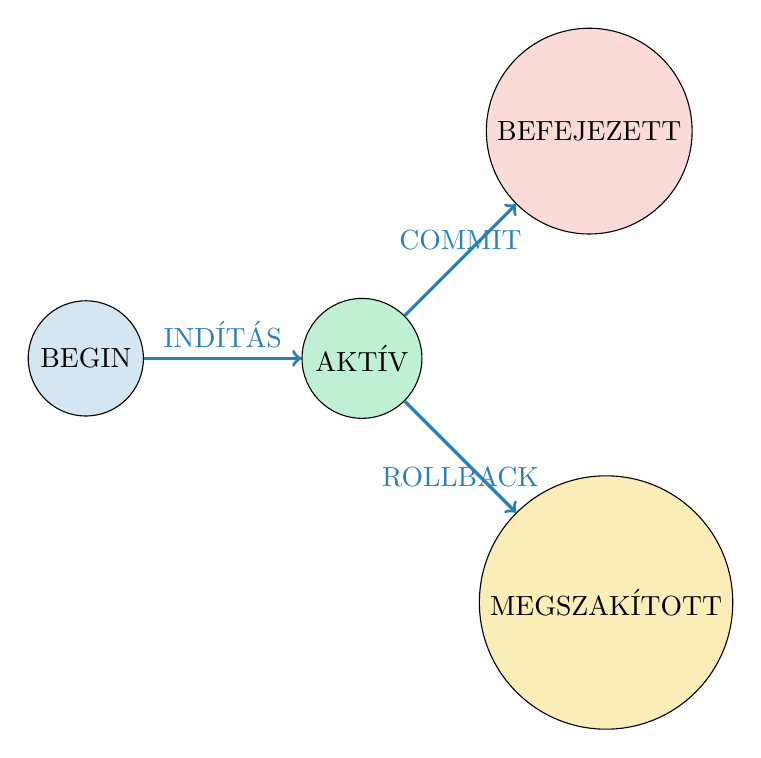
\begin{tikzpicture}[node distance=2cm, auto]
    \node[circle, draw, fill=primaryblue!20] (begin) {BEGIN};
    \node[circle, draw, fill=success!30, right=of begin] (active) {AKTÍV};
    \node[circle, draw, fill=accent!20, above right=of active] (commit) {BEFEJEZETT};
    \node[circle, draw, fill=warning!30, below right=of active] (abort) {MEGSZAKÍTOTT};
    
    \draw[->, line width=1.2pt, color=primaryblue] (begin) -- (active) node[midway, above] {INDÍTÁS};
    \draw[->, line width=1.2pt, color=primaryblue] (active) -- (commit) node[midway, above] {COMMIT};
    \draw[->, line width=1.2pt, color=primaryblue] (active) -- (abort) node[midway, below] {ROLLBACK};
\end{tikzpicture}
\end{center}
\end{block}
\end{frame}

\begin{frame}{Egyidejűség-vezérlés}
\begin{block}{Zárolás Kezelő Implementáció}
\begin{itemize}
    \item \textbf{Zárolás Típusok}: Megosztott (S) és Kizárólagos (X) zárolások
    \item \textbf{Zárolás Granularitás}: Rekord-szintű és tábla-szintű zárolás
    \item \textbf{Holtpont Megelőzés}: Időkorlát-alapú megoldás
    \item \textbf{Zárolás Kompatibilitási Mátrix}:
\end{itemize}
\end{block}

\begin{center}
\begin{tabular}{|c|c|c|}
\hline
& \textbf{Megosztott} & \textbf{Kizárólagos} \\
\hline
\textbf{Megosztott} & ✓ & ✗ \\
\hline
\textbf{Kizárólagos} & ✗ & ✗ \\
\hline
\end{tabular}
\end{center}

\begin{alertblock}{Haladó Funkció}
A pyHMSSQL \textbf{szándék zárolásokat} (IS, IX) implementál hierarchikus zároláshoz, lehetővé téve hatékony többszintű egyidejűség-vezérlést.
\end{alertblock}
\end{frame}

\section{Halmazműveletek}

\begin{frame}{Halmazműveletek Implementációja}
\begin{block}{Támogatott Halmazműveletek}
\begin{itemize}
    \item \textbf{UNION}: Eredmények kombinálása, duplikátumok eliminálása
    \item \textbf{INTERSECT}: Közös rekordok visszaadása halmazok között
    \item \textbf{EXCEPT}: Bal halmazban lévő, de jobb halmazban nem lévő rekordok visszaadása
\end{itemize}
\end{block}

\begin{block}{Implementációs Stratégia}
\begin{enumerate}
    \item \textbf{Allekérdezések Végrehajtása}: Bal és jobb operandusok független végrehajtása
    \item \textbf{Eredmény Normalizálás}: Közös rekord formátumra konvertálás
    \item \textbf{Halmaz Művelet Logika}: Matematikai halmazelmélet alkalmazása
    \item \textbf{Duplikátum Eliminálás}: Hash-alapú deduplikáció UNION-hoz
\end{enumerate}
\end{block}

\begin{block}{Komplexitás Elemzés}
\begin{align}
\text{UNION Költség} &= |L| + |R| + \text{Rendezés/Hash Költség} \\
\text{INTERSECT Költség} &= |L| \times \log|R| \text{ (ha indexelt)} \\
\text{EXCEPT Költség} &= |L| \times \log|R| \text{ (ha indexelt)}
\end{align}
\end{block}
\end{frame}

\section{Tárolási Motor}

\begin{frame}{Tárolási Architektúra}
\begin{block}{Tárolási Komponensek}
\begin{itemize}
    \item \textbf{Katalógus Kezelő}: Metaadat és séma kezelés
    \item \textbf{Puffer Pool Kezelő}: Memória kezelés oldalakhoz
    \item \textbf{Index Kezelő}: B+ fa perzisztencia és kezelés
    \item \textbf{Fájl Kezelő}: Alacsony szintű fájlműveletek
\end{itemize}
\end{block}

\begin{block}{Adat Szervezés}
\begin{itemize}
    \item \textbf{Adatbázis Fájlok}: Külön könyvtárak adatbázisonként
    \item \textbf{Tábla Fájlok}: Bináris szerializáció séma metaadatokkal
    \item \textbf{Index Fájlok}: B+ fa szerializáció hatékony hozzáféréssel
    \item \textbf{Napló Fájlok}: Előre írt naplózás helyreállításhoz
\end{itemize}
\end{block}

\begin{alertblock}{Teljesítmény Optimalizálás}
Puffer pool \textbf{LRU kiszorítással} és \textbf{oldal rögzítéssel} biztosítja, hogy a gyakran elért adatok memóriában maradjanak.
\end{alertblock}
\end{frame}

\begin{frame}{Séma Kezelés}
\begin{block}{Tárolt Katalógus Információk}
\begin{itemize}
    \item \textbf{Adatbázis Metaadatok}: Létrehozási idő, tulajdonos, tulajdonságok
    \item \textbf{Tábla Sémák}: Oszlop definíciók, megszorítások, indexek
    \item \textbf{Index Definíciók}: B+ fa konfiguráció és statisztikák
    \item \textbf{Felhasználói Információk}: Hitelesítési és jogosultsági adatok
    \item \textbf{Nézet Definíciók}: Tárolt lekérdezés szöveg és függőségek
\end{itemize}
\end{block}

\begin{block}{Kis- és Nagybetű Érzékenység Kezelés}
A pyHMSSQL \textbf{kis- és nagybetű érzéketlen} tábla és oszlop név feloldást implementál, miközben megőrzi az \textbf{eredeti betűméretet} a tárolásban:\\

\texttt{SELECT * FROM Customers} $\rightarrow$ \texttt{customers}

Ez \textbf{SQL szabvány megfelelőséget} biztosít a használhatóság fenntartása mellett.
\end{block}
\end{frame}

\section{Haladó Funkciók}

\begin{frame}{Nézetek és Virtuális Táblák}
\begin{block}{Nézet Implementáció}
\begin{itemize}
    \item \textbf{Nézet Definíció Tárolás}: Elemzett lekérdezés tárolva a katalógusban
    \item \textbf{Lekérdezés Helyettesítés}: Nézet hivatkozások lecserélve tárolt lekérdezéssel
    \item \textbf{Rekurzív Feloldás}: Támogatás nézetekre hivatkozó nézetekhez
    \item \textbf{Biztonsági Integráció}: Nézet-alapú hozzáférés-vezérlés
\end{itemize}
\end{block}

\begin{block}{Nézet Feldolgozási Algoritmus}
\begin{enumerate}
    \item Nézet hivatkozást tartalmazó lekérdezés elemzése
    \item Nézet definíció lekérése a katalógusból
    \item Nézet hivatkozás helyettesítése tárolt lekérdezéssel
    \item További WHERE feltételek alkalmazása
    \item Módosított lekérdezés végrehajtása
\end{enumerate}
\end{block}

\begin{alertblock}{Optimalizálási Lehetőség}
Nézet materializálás és inkrementális karbantartás jelentősen javíthatná a lekérdezési teljesítményt összetett nézetekhez.
\end{alertblock}
\end{frame}

\begin{frame}{Replikáció és Magas Elérhetőség}
\begin{block}{Replikációs Architektúra}
\begin{itemize}
    \item \textbf{Mester-Szolga Topológia}: Elsődleges szerver többszörös replikákkal
    \item \textbf{Szinkronizációs Módok}: Szinkron, félszinkron, aszinkron replikáció
    \item \textbf{Konfliktus Megoldás}: Utolsó-író-győz időbélyeg rendezéssel
    \item \textbf{Failover Támogatás}: Automatikus replika előléptetés elsődlegessé
\end{itemize}
\end{block}

\begin{block}{Replikációs Konzisztencia Szintek}
\begin{enumerate}
    \item \textbf{Szinkron}: Minden replikának nyugtáznia kell commit előtt
    \item \textbf{Félszinkron}: Konfigurálható számú replikának kell nyugtáznia
    \item \textbf{Aszinkron}: Elsődleges azonnal commitol, replikák később frissülnek
\end{enumerate}
\end{block}

\begin{block}{CAP Tétel Kompromisszumok}
A pyHMSSQL lehetővé teszi a \textbf{Konzisztencia vs Elérhetőség} kompromisszumok konfigurálását replikációs mód kiválasztás révén.
\end{block}
\end{frame}

\section{Teljesítmény Elemzés}

\begin{frame}{Lekérdezés Optimalizálás Hatása}
\begin{block}{Optimalizálási Technikák Teljesítménye}
\begin{itemize}
    \item \textbf{Index Használat}: 10-1000x teljesítményjavulás szelektív lekérdezésekhez
    \item \textbf{Join Újrarendezés}: 2-10x javulás többtáblás összekapcsolásokhoz
    \item \textbf{Predikátum Lenyomás}: 50-90\% csökkenés köztes eredmény méretben
    \item \textbf{Kötegelt Műveletek}: 10-100x javulás tömeges beszúrásokhoz
\end{itemize}
\end{block}

\begin{block}{B+ Fa Teljesítmény}
\begin{align}
\text{Keresési Idő} &= O(\log_m n) \text{ ahol } m \text{ az elágazási tényező} \\
\text{Tartomány Lekérdezés} &= O(\log_m n + k) \text{ ahol } k \text{ az eredmény mérete} \\
\text{Tipikus Elágazási Tényező} &\approx 100-500 \text{ (kulcs mérettől függ)}
\end{align}
\end{block}

\begin{alertblock}{Valós Teljesítmény}
Megfelelő indexeléssel a pyHMSSQL \textbf{milliónyi rekordot} képes kezelni másodperc alatti lekérdezési válaszidőkkel általános hardveren.
\end{alertblock}
\end{frame}

\begin{frame}{Skálázhatósági Elemzés}
\begin{block}{Vertikális Skálázási Karakterisztikák}
\begin{itemize}
    \item \textbf{Memória}: Puffer pool lineárisan skálázódik az elérhető RAM-mal
    \item \textbf{CPU}: Párhuzamos lekérdezés végrehajtás összetett műveletekhez
    \item \textbf{Tárolás}: Hatékony B+ fa struktúra minimalizálja I/O-t
\end{itemize}
\end{block}

\begin{block}{Horizontális Skálázás (Replikáció)}
\begin{itemize}
    \item \textbf{Olvasási Skálázás}: Lineáris javulás olvasási replikákkal
    \item \textbf{Írási Skálázás}: Korlátozott szinkronizációs követelményekkel
    \item \textbf{Földrajzi Elosztás}: Támogatás távoli replikákhoz
\end{itemize}
\end{block}

\begin{block}{Szűk Keresztmetszet Elemzés}
\begin{enumerate}
    \item \textbf{I/O Korlátozott}: Megoldva indexeléssel és puffer poolokkal
    \item \textbf{CPU Korlátozott}: Kezelve lekérdezés optimalizálással
    \item \textbf{Hálózat Korlátozott}: Minimalizálva hatékony protokollokkal
\end{enumerate}
\end{block}
\end{frame}

\section{Összehasonlítás Gyártási Rendszerekkel}

\begin{frame}{Funkció Összehasonlítás}
\begin{center}
\begin{tabular}{|l|c|c|c|c|}
\hline
\textbf{Funkció} & \textbf{pyHMSSQL} & \textbf{PostgreSQL} & \textbf{MySQL} & \textbf{SQLite} \\
\hline
ACID Tranzakciók & ✓ & ✓ & ✓ & ✓ \\
B+ Fa Indexek & ✓ & ✓ & ✓ & ✓ \\
Idegen Kulcsok & ✓ & ✓ & ✓ & ✓ \\
Nézetek & ✓ & ✓ & ✓ & ✓ \\
Tárolt Eljárások & ✓ & ✓ & ✓ & ✗ \\
Replikáció & ✓ & ✓ & ✓ & ✗ \\
REST API & ✓ & ✗ & ✗ & ✗ \\
Egyedi Aggregátumok & ✓ & ✓ & ✓ & ✗ \\
Lekérdezés Optimalizálás & ✓ & ✓ & ✓ & ✓ \\
\hline
\end{tabular}
\end{center}

\begin{alertblock}{Egyedi Funkciók}
A pyHMSSQL több egyedi funkciót tartalmaz, mint \textbf{beépített REST API}, \textbf{matematikai aggregátumok (GCD)}, és \textbf{integrált vizualizációs eszközök}.
\end{alertblock}
\end{frame}

\begin{frame}[c]
\begin{center}
{\Huge Köszönöm}

\vspace{1cm}

\vspace{1cm}

\textit{pyHMSSQL: Egy teljes, gyártásra kész adatbázis-kezelő rendszer, amely az adatbázis elmélet teljes spektrumát demonstrálja a gyakorlatban.}
\end{center}
\end{frame}

\end{document}